\section{Implementazione generatore SVG}

La funzione principale del linguaggio cUml è quella di permettere la creazione 
di diagrammi UML partendo da un modello dati e uno schema di layout.
Come dice il nome del programma il formato prescelto per l'esportazione è SVG
\cite{svg_website} ovvero un formato vettoriale creato dal W3C
\cite{w3c_website} basato su XML.
La generazione della grafica avviene in due passi principali:
\begin{itemize}
  \item lettura e controllo del modello ad oggetti;
  \item lettura e applicazione dei parametri di layout agli oggetti;
\end{itemize}

Al termine di queste due fasi abbiamo a disposizione una rappresentazione degli
oggetti con i dettagli che permettono il corretto posizionamento all'interno
dello spazio della grafica.
L'unica cosa che rimane da fare a questo punto è la generazione del codice vero
e proprio che costituisce SVG. Per questa fase la scelta dello strumento da
utilizzare è caduta su Apache Velocity \cite{apache_velocity_website}, un motore di 
template parametrico scritto in linguaggio Java che ha permesso di semplificare
di molto il lavoro da compiere.

\subsection{Apache Velocity}
Velocity è uno strumento molto potente e possiede un suo linguaggio interno per
realizzare cicli e controlli condizionali direttamente all'interno del codice
del template, in questo modo è stato semplice creare dei modelli dinamici di
codice che si adattassero allo stato effettivo degli oggetti da disegnare.

\subsection{La gestione dell'esportazione}
Il template è praticamente tutto codice SVG con inclusi controlli condizionali e
cicli per l'adattamento alle condizioni dell'oggetto da disegnare. Per
semplicità e pulizia, il template è stato spezzato in diversi sotto-template che
vengono richiamati ognuno dall'oggetto che ne fa uso.
Nel modello utilizzato da cUml2Svg la struttura è costituita da diversi oggetti:
\begin{itemize}
  \item SVGExporter: è l'oggetto principale che comanda l'esportazione prendendo
  come parametro un Diagramma e i dettagli di esportazione ovvero il nome del
  file da creare e il percorso dove trovare i template di esportazione;
  \item Diagram: come si può intuire è il componente principale del diagramma
  ovvero l'oggetto che contiene tutti i componenti che costituiscono il modello;
  \item Group: rappresenta il blocco logico di esportazione del modello ed è
  quello che raggruppa le classi permettendone la disposizione;
  \item Class: rappresenta l'oggetto vero e proprio, ovvero il componente
  principale del diagramma con attributi e metodi;
  \item Relation: serve per rappresentare le connessioni tra le classi;
\end{itemize}
L'esportazione avviene chiamando il metodo \lstinline{export()} di SVGExporter,
questo provvede a chiamare il metodo \lstinline{render()} del diagramma il quale
ricorsivamente chiama lo stesso metodo di tutti gli oggetti (gruppi e classi)
che si occupano poi di caricare e compilare i template.
Al termine delle chiamate a \lstinline{render()} il controllo ritorna ad
SVGExporter che effettua la scrittura su file del grafico creato.

\subsection{Un esempio di SVG generato}
Il risultato dell'esportazione come detto è SVG, ovvero codice XML che
rappresenta gli oggetti grafici. Quello di seguito è un esempio di codice
generato da uno degli esempi presenti nel capitolo relativo, nello specifico
l'esempio 2.

\begin{lstlisting}[language=xml, caption={Un esempio di codice SVG generato}]
<?xml version="1.0" standalone="no"?>
<!DOCTYPE svg PUBLIC "-//W3C//DTD SVG 1.1//EN" 
  "http://www.w3.org/Graphics/SVG/1.1/DTD/svg11.dtd">
<svg version="1.1"
     width="29.7cm" height="21cm" viewBox="-150 -150 1478 490"
     xmlns="http://www.w3.org/2000/svg">
  <desc>Export of </desc>
  <defs id="definitions">
    <marker
       refX="0"
       refY="0"
       orient="auto"
       style="overflow:visible"
       id="Use">
      <path
         d="M -35.0,11.5 L -0.0,0.0 L -35.0,-11.5 L 
-35.0,11.5 z "
         transform="scale(0.9,0.9)"
         style="fill-rule:evenodd;stroke:#000000;
stroke-width:1pt;marker-start:none"
      />
    </marker>
...
  </defs>
  <g transform="translate(0,0)" >
  <rect
    width="414"
    height="152"
    rx="0"
    ry="0"
    x="0"
    y="0"
    style="fill:#fff6d5;stroke:#800080;stroke-width:1.25;
stroke-miterlimit:4;stroke-dasharray:none"
  />
  <text
    x="20"
    y="38"
    style="font-size:28px;font-style:normal;font-weight:normal;
text-align:start;text-anchor:start;fill:#000000;fill-opacity:1;
stroke:none;stroke-width:1px;stroke-linecap:butt;
stroke-linejoin:miter;stroke-opacity:1;
font-family:Bitstream Vera Sans Mono">
    <tspan
      x="227"
      y="38"
      style="font-size:28px;text-align:center;
text-anchor:middle;font-family:Bitstream Vera Sans Mono">
      org.example.Classe1
     </tspan>
  </text>
  <path
    d="M 0,48 L 414,48"
    style="fill:none;fill-rule:evenodd;stroke:#800080;
stroke-width:1px;stroke-linecap:butt;stroke-linejoin:miter;
stroke-opacity:1"
  />
  <text
    x="20"
    y="76"
    style="font-size:28px;font-style:normal;font-weight:normal;
text-align:start;text-anchor:start;fill:#000000;fill-opacity:1;
stroke:none;stroke-width:1px;stroke-linecap:butt;
stroke-linejoin:miter;stroke-opacity:1;
font-family:Bitstream Vera Sans Mono">
      +x:int=0
  </text>
  <path
         d="M 0,86 L 414,86"
     style="fill:none;fill-rule:evenodd;stroke:#800080;
stroke-width:1px;stroke-linecap:butt;
stroke-linejoin:miter;stroke-opacity:1"
  />
  <text
    x="20"
    y="114"
    style="font-size:28px;font-style:normal;font-weight:normal;
text-align:start;text-anchor:start;fill:#000000;fill-opacity:1;
stroke:none;stroke-width:1px;stroke-linecap:butt;
stroke-linejoin:miter;stroke-opacity:1;
font-family:Bitstream Vera Sans Mono">
      +print():void
  </text>
</g>
...
</svg>
\end{lstlisting}

L'esempio è stato accorciato per brevità, comunque è possibile notare 
che tutto il modello viene scomposto e rappresentato in gruppi
(\lstinline{<g></g>}), rettangoli (\lstinline{<rect></rect>}), testo 
(\lstinline{<text><tpath></tpath></text>}) e linee (\lstinline{<path></path>}).
Da questi elementi prende vita il disegno finale del diagramma:

\begin{figure}[htp]
\begin{center}
  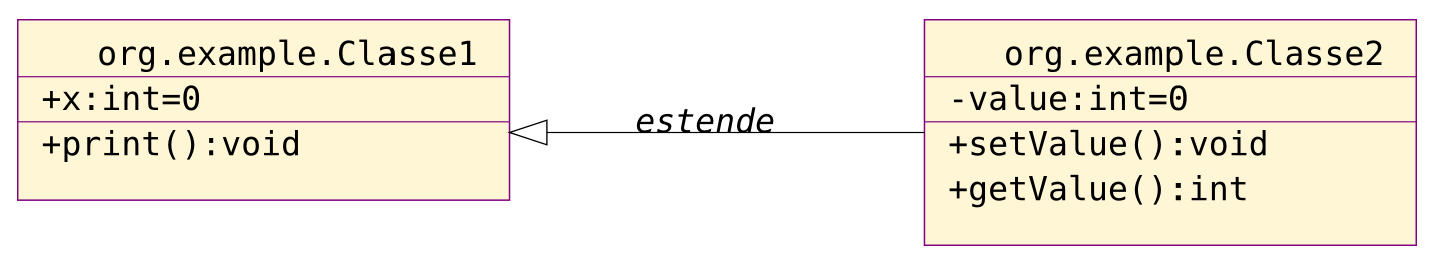
\includegraphics[width=0.9\textwidth]{img/esempio2}
  \caption[labelInTOC]{Risultato dell'esportazione del codice dell'esempio 2}
\end{center}
\end{figure}

